\documentclass[12pt]{article}
\usepackage[francais]{babel}
\usepackage[table]{xcolor}
\usepackage{graphicx}
\usepackage[T1]{fontenc}
\usepackage{lmodern}
\usepackage{float}
\usepackage{pdfpages}
\usepackage[left=2cm,right=2cm,top=2cm,bottom=2cm]{geometry}
%============================acronymes===================================
\usepackage[nopostdot,nogroupskip,style=super,nonumberlist,toc,automake,toc]{glossaries} %Load glossaries package
\makeglossaries

%Here we define a set of example acronyms
\newglossaryentry{Ape}{name={APE},description={Activité Principale Exercée}}
\newglossaryentry{Ca}{name={CA},description={Chiffre d’Affaires}}
\newglossaryentry{Cpv}{name={CPV},description={Common Procurement Vocabulary}}

\newglossaryentry{Ebe}{name={EBE},description={Excédent Brut d'Exploitatione}}
\newglossaryentry{Sigma}{name={SIGMA},description={Système Informatique de Gestion et de Management des Achats}}
\newglossaryentry{Siret}{name={SIRET},description={Système d’Identification du Répertoire des Établissements}}

%===============================================================
%partie concernant la gestion des entêtes/footer
\usepackage{fancyhdr}
\pagestyle{fancy}
\usepackage{lastpage}
\renewcommand\headrulewidth{1pt}
\fancyhead[L]{Master 1 GIL - Projet : Théorie des jeux}
\fancyhead[R]{Université de Rouen}
\renewcommand\footrulewidth{1pt}
\fancyfoot[L]{Mini projet THJ}
\fancyfoot[C]{
	\textbf{Page \thepage/\pageref{LastPage}}}
\fancyfoot[R]{2022/2023}
%fin

\begin{document} 
	\thispagestyle{empty}
	
	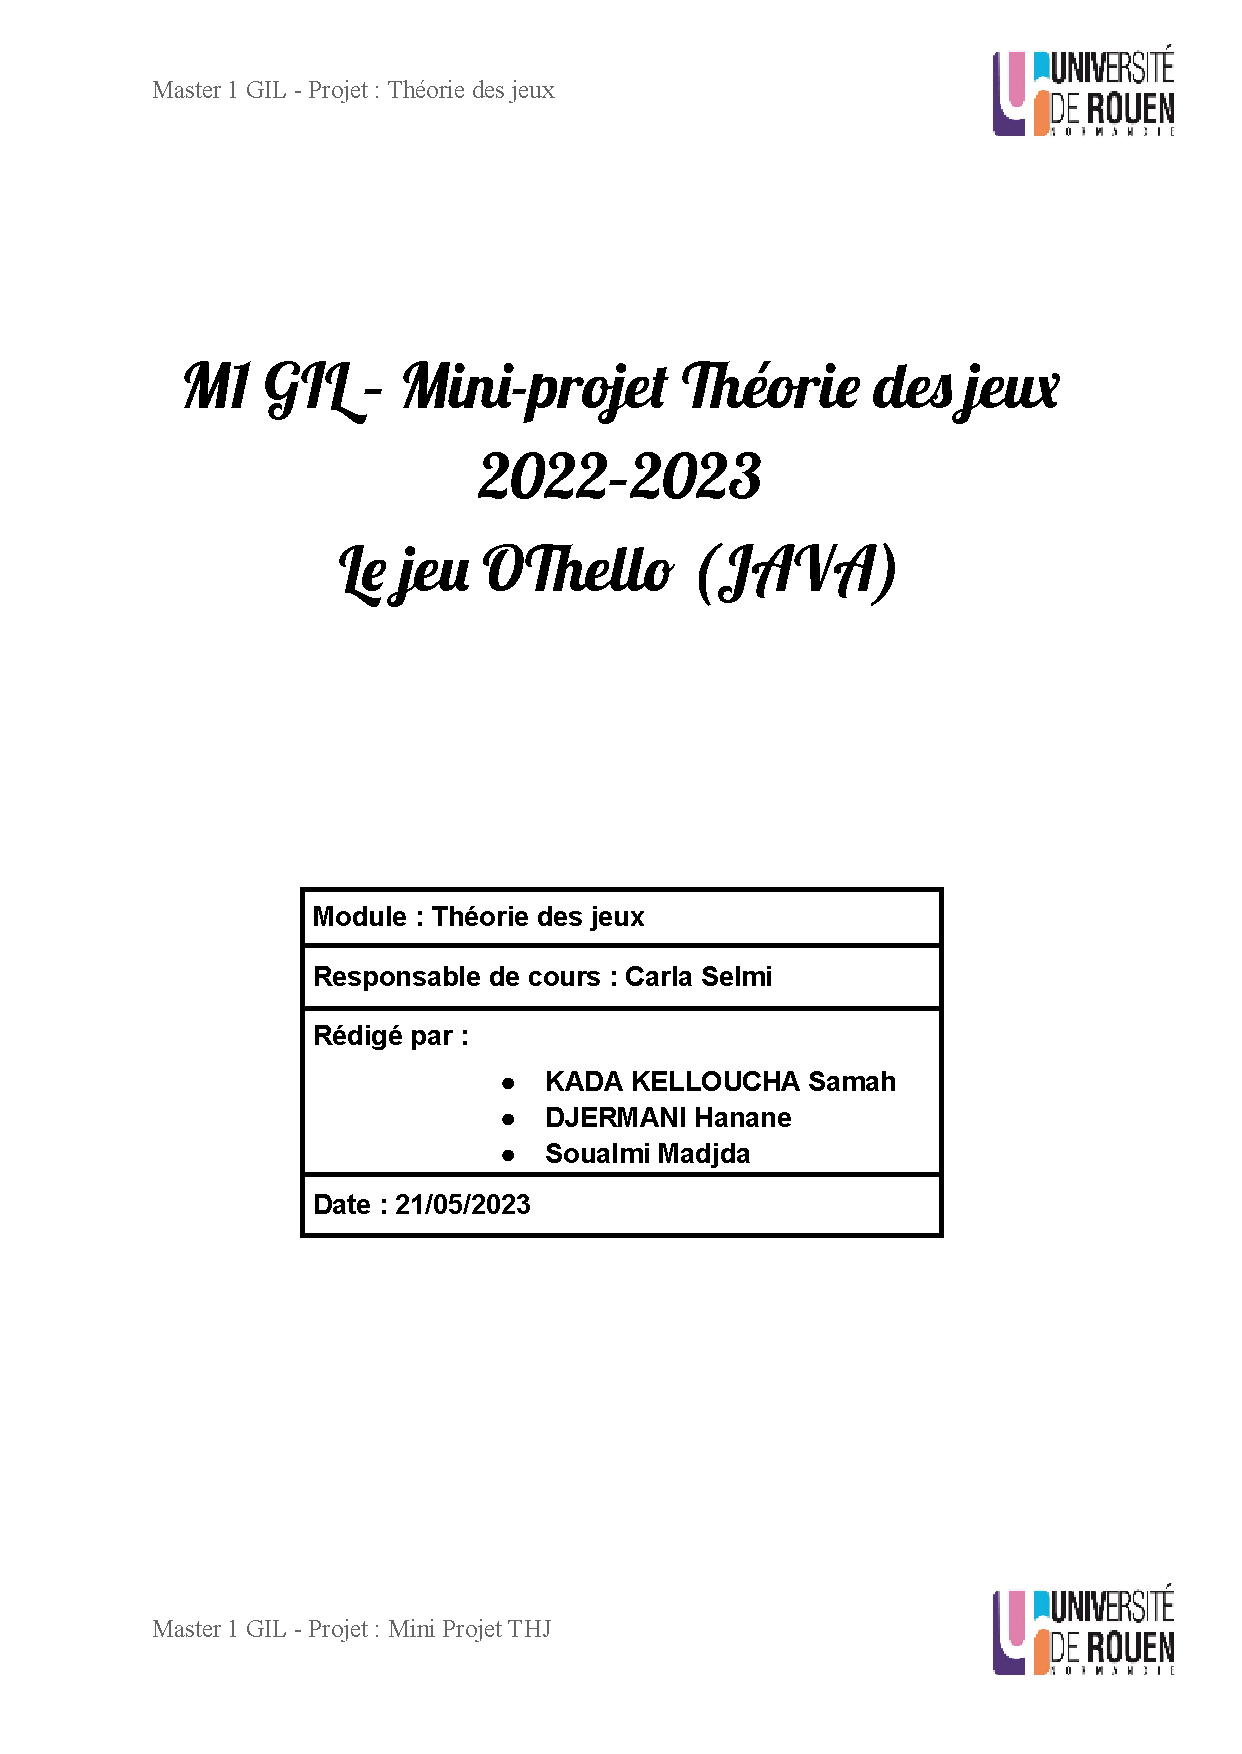
\includepdf{page.pdf}
	
	\newpage
	\tableofcontents
	\newpage
	\listoffigures
	\newpage
	\printglossary[title={Liste des Abbréviations}] %Generate List of Abbreviations
	\newpage
	%--------------------------Début de rapport ----------------------------
	\section{Introduction}
	\subsection{Présentation du jeu Othello et de son contexte:}



Othello, également connu sous le nom de Reversi, est un jeu de stratégie passionnant qui oppose deux joueurs. Il se joue sur un plateau de 8x8 cases, avec 64 pions bicolores réversibles. L'objectif du jeu est de capturer le plus grand nombre possible de pions de son adversaire en les encadrant avec ses propres pions. Les règles du jeu sont simples, mais les possibilités tactiques sont nombreuses, ce qui en fait un défi stimulant pour les joueurs de tous niveaux.

Dans Othello, les joueurs doivent faire preuve de réflexion stratégique, de planification à long terme et de capacité d'anticipation pour prendre les bonnes décisions. Chaque coup peut avoir des conséquences importantes sur le déroulement de la partie, car les pions retournés peuvent changer la configuration du plateau et influencer les possibilités de jeu.

Ce jeu de société classique a été inventé dans les années 1880 et est depuis devenu populaire dans le monde entier. Il est souvent utilisé comme moyen d'entraînement pour développer les compétences de pensée critique et de prise de décision.

\subsection{Objectifs du projet:}

Le principal objectif de ce projet est de développer une version informatisée du jeu Othello avec une interface graphique conviviale. Cette version permettra aux utilisateurs de jouer contre l'ordinateur en choisissant différents niveaux de difficulté. Le programme implémentera également plusieurs stratégies de jeu, telles que Minimax, NegaMax, Alpha-Beta, NegaAlphaBeta, SSS* et A*, afin de fournir une expérience de jeu variée et stimulante.\\

\textbf{Les objectifs spécifiques du projet comprennent :}

\begin{itemize}
	\item Implémenter les règles du jeu Othello et les mécanismes de jeu associés.
	\item Concevoir et développer une interface graphique attrayante pour le jeu.
	\item Programmer les différentes stratégies de jeu pour l'ordinateur.
	\item Permettre aux utilisateurs de sélectionner la difficulté et de jouer contre l'ordinateur.
	\item Réaliser des tests approfondis pour s'assurer du bon fonctionnement du jeu.
\end{itemize}

\begin{figure}[H]
	\centering
	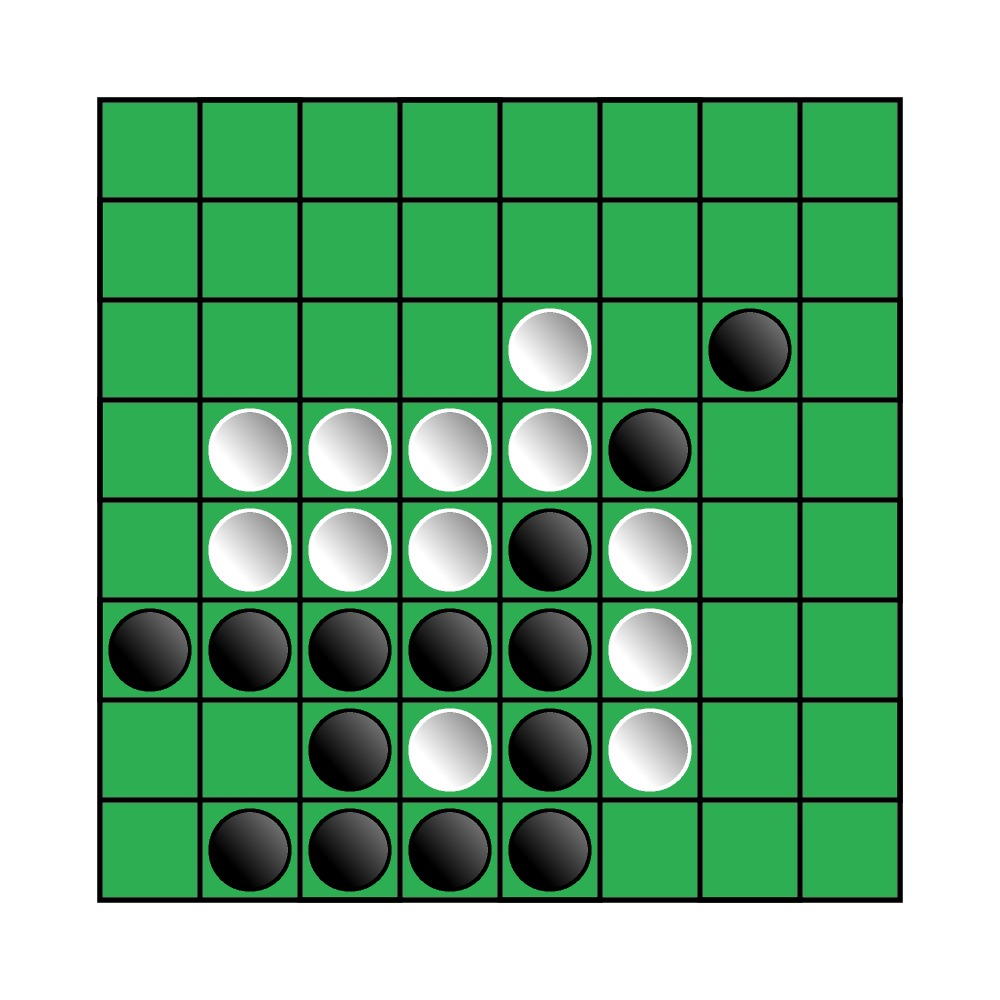
\includegraphics[scale=0.2]{img/othello}
	\caption{Le jeu Othello}
	\label{othello figure}
\end{figure}
\newpage
	\section{Analyse des besoins}	
	\subsection{Description des fonctionnalités principales du jeu Othello}
Le jeu Othello développé dans le cadre de ce projet comprendra les fonctionnalités suivantes :

\paragraph{Interface graphique conviviale :} Le jeu disposera d'une interface graphique intuitive et esthétiquement agréable. Les utilisateurs pourront facilement naviguer dans le jeu, visualiser le plateau de jeu et effectuer leurs coups.

\paragraph{Règles du jeu :} Le programme implémentera les règles officielles du jeu Othello, notamment la pose des pions, le retournement des pions adverses et les contraintes de mouvement. Les joueurs aurons toujours l'accès au règles et des actions autorisées à chaque tour.

\paragraph{Modes de jeu :} Les utilisateurs auront la possibilité de jouer contre l'ordinateur à différents niveaux de difficulté. Le jeu offrira également un mode de jeu à deux joueurs, permettant à deux personnes de s'affronter sur le même appareil.

\paragraph{Stratégies de jeu :} Le jeu intégrera plusieurs stratégies de jeu pour l'ordinateur, telles que Minimax, NegaMax, Alpha-Beta, NegaAlphaBeta, SSS* et A*. Chaque stratégie aura un niveau de difficulté différent, offrant ainsi aux joueurs un défi adapté à leur niveau de compétence.

\paragraph{Aide et conseils :} Pour aider les joueurs débutants, le jeu proposera des fonctionnalités d'aide et de conseils.



\subsection{Les règles de jeu Othello}
 Les règles du jeu Othello, également appelé Reversi, sont les suivantes :\\
\begin{itemize}

	
	\item	Le jeu est joué sur un plateau de 8x8 cases.
	\item	Chaque joueur a un certain nombre de pions de sa couleur. Au début du jeu, deux pions noirs et deux pions blancs sont placés dans les cases centrales du plateau.
	\item Les joueurs jouent chacun leur tour. Le joueur avec les pions noirs commence la partie.
		\item Un coup consiste à placer un pion de sa propre couleur sur une case vide du plateau.
		\item Pour que le coup soit valide, le joueur doit placer son pion de manière à ce qu'il encercle un ou plusieurs pions adverses entre le pion placé et un autre pion de sa couleur déjà présent sur le plateau.
 	\item	Les pions encerclés sont alors retournés et deviennent de la couleur du joueur qui vient de jouer.
	\item	Si un joueur ne peut pas jouer, il passe son tour. Si les deux joueurs passent leur tour consécutivement, la partie se termine.
		\item Le jeu se termine lorsque toutes les cases sont occupées ou qu'aucun des deux joueurs ne peut jouer.
	\item	Le joueur qui a le plus de pions de sa couleur sur le plateau à la fin de la partie est déclaré vainqueur.
\end{itemize}
\section{Présentation de l'architecture générale du programme:}
Le programme du jeu Othello est conçu en utilisant une architecture orientée objet. Il est divisé en plusieurs classes et modules qui interagissent entre eux pour assurer le bon fonctionnement du jeu. L'architecture générale du programme se compose de 4 pacquages principaux :

\subsection{Model:}La classe Board représente le plateau de jeu et contient une grille de cases (modelBoardSquares). Elle initialise le plateau avec les pions de départ et fournit des méthodes pour jouer un coup, vérifier si la partie est terminée et obtenir les successeurs possibles pour un joueur.

La classe Direction est une énumération qui définit les différentes directions possibles pour un mouvement sur le plateau.L'énumération Pawn représente les différentes couleurs de pions possibles dans le jeu.La classe Player représente un joueur et contient des informations telles que la couleur de son pion, son statut (joueur humain ou ordinateur), son score et les mouvements valides qu'il peut effectuer.La classe Sound permet de jouer des fichiers audio dans le jeu.La classe Square représente une case sur le plateau de jeu et contient son état (vide, occupé par un pion noir ou un pion blanc).L'énumération State représente les différents états possibles pour une case (vide, occupé par un pion noir ou un pion blanc) et fournit une méthode pour obtenir l'état opposé.

\subsection{View:} la vue de projet représentée par l'interface graphique du jeu, où les joueurs peuvent voir le plateau de jeu, les pions, les scores, les indications visuelles, les messages, etc. La vue interagirait avec le contrôleur pour recevoir les commandes de l'utilisateur (par exemple, cliquer sur une case du plateau) et mettre à jour le modèle en conséquence. Elle serait également responsable de l'affichage des animations lors des mouvements de pions ou de tout autre effet visuel.

\subsection{Controller:}ce pacquage contient Les classes qui sont utilisées pour contrôler le jeu Othello. La classe `\textbf{BoardListener}` implémente l'interface `\textbf{MouseListener}` pour gérer les événements de souris sur le plateau de jeu. Elle détecte les clics de souris sur les cases du plateau, effectue des vérifications et met à jour l'état du jeu en fonction des actions du joueur. La classe `\textbf{MenuListener}` implémente également `\textbf{MouseListener}` et gère les événements de souris sur les menus du jeu, tels que l'aide et les règles du jeu. La classe `\textbf{Move}` contient des méthodes pour générer des mouvements valides, changer l'état des cases et mettre à jour les scores des joueurs. La classe `\textbf{Play}` est responsable du démarrage du jeu, de l'initialisation des joueurs, du plateau et de la vue, et de la gestion des paramètres du jeu tels que le pion du joueur, le niveau de difficulté et l'algorithme utilisé.

\subsection{Strategy:}Les différentes stratégies de jeu, telles que Minimax, NegaMax, Alpha-Beta, NegaAlphaBeta, SSS* et A*, sont implémentées dans des classes séparées. Chaque stratégie a ses propres algorithmes de recherche, d'évaluation et de prise de décision.


\section{Les stratégies de jeu demandés}
	    \subsection{Min-Max [\ref{Algorithme MINIMAX}] :} Cet algorithme est une technique de recherche de l'arbre de jeu pour les jeux à deux joueurs. Il consiste à maximiser le gain possible du joueur en minimisant le gain possible de son adversaire. Pour chaque coup possible, il explore tous les coups suivants possibles et évalue le score obtenu pour le joueur en question. Ensuite, il choisit le coup qui maximise le score pour le joueur .
	    
	    
	    
	    \begin{figure}[H]
	    	\centering
	    	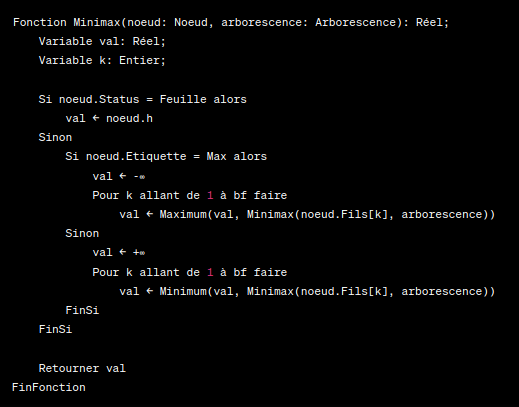
\includegraphics[scale=0.55]{img/minimax}
	    	\caption{Algorithme MINIMAX }
	    	\label{Algorithme MINIMAX}
	    \end{figure}
	\subsection{NégaMax[\ref{Algorithme NégaMINIMAX}]:}L'algorithme Négamax est une variante de l'algorithme Minimax utilisé pour la recherche de coups optimaux dans les jeux à deux joueurs avec information parfaite, tels que les échecs, les dames et Othello.
	
	 \begin{figure}[H]
		\centering
		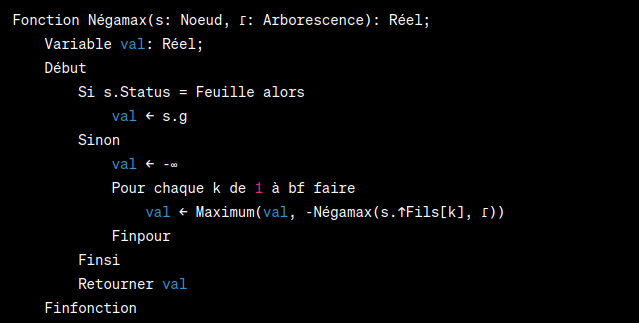
\includegraphics[scale=0.55]{img/negamax.png}
		\caption{Algorithme NÉGAMAX }
		\label{Algorithme NégaMINIMAX}
	\end{figure}
	
	
	
	
	\subsection{Alpha-Beta [\ref{Algorithme ALPHABETA}] :} C'est une amélioration de l'algorithme Min-Max qui permet de réduire considérablement le nombre de nœuds évalués. Au lieu d'explorer tous les nœuds, l'algorithme Alpha-Beta utilise une technique de coupure pour éviter d'explorer des branches qui ne contribuent pas au résultat final. L'algorithme utilise deux valeurs, alpha et beta, pour suivre les valeurs minimales et maximales possibles.
	
	   
	\begin{figure}[H]
		\centering
		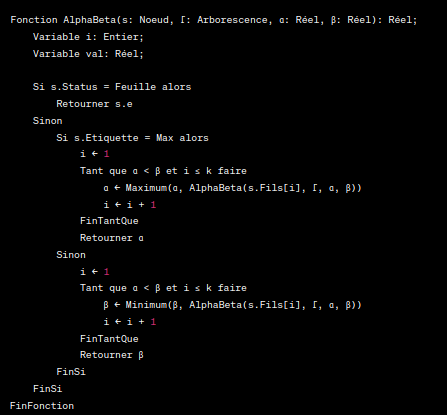
\includegraphics[scale=0.7]{img/alphabeta}
		\caption{Algorithme ALPHABETA }
		\label{Algorithme ALPHABETA}
	\end{figure}
	
	
		
\subsection{NégaAlphaBeta [\ref{Algorithme NégaAlphaBeta}]: }C'est une variation de l'algorithme Alpha-Beta qui est souvent utilisée pour les jeux à somme nulle comme l'othello. Il est similaire à l'algorithme Alpha-Beta, mais utilise une valeur de score négative pour le joueur adverse.
	
	
		   
	\begin{figure}[H]
		\centering
		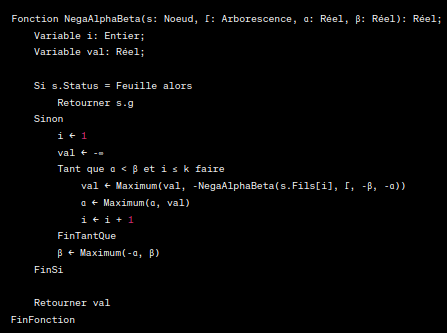
\includegraphics[scale=0.7]{img/negaalphabeta}
		\caption{Algorithme NégaAlphaBeta }
		\label{Algorithme NégaAlphaBeta}
	\end{figure}
	
	\subsection{SSS* [\ref{Algorithme SSS*}] :} C'est une amélioration de l'algorithme A* qui utilise une liste ouverte de nœuds pour stocker les nœuds qui doivent encore être évalués. Contrairement à l'algorithme A*, qui utilise une file de priorité, SSS* utilise une liste liée. Cela permet de réduire le temps de calcul en évitant les opérations de tri nécessaires pour maintenir l'ordre de priorité dans une file de priorité.
	
		\begin{figure}[H]
		\centering
		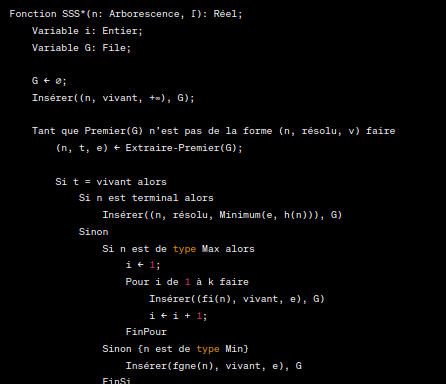
\includegraphics[scale=0.7]{img/sss1}
	\end{figure}
		\begin{figure}[H]
		\centering
		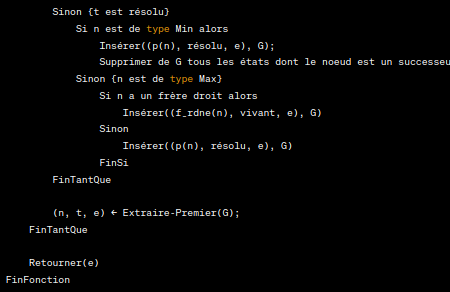
\includegraphics[scale=0.7]{img/sss2}
		\caption{Algorithme SSS* }
		\label{Algorithme SSS*}
	\end{figure}
	
\subsection{A* [\ref{Algorithme A*}] :} C'est un algorithme de recherche de chemin qui peut être utilisé pour trouver le chemin optimal entre deux points dans un graphe. Il utilise une fonction heuristique pour estimer le coût du chemin restant à partir du nœud actuel. L'algorithme explore les nœuds en fonction de leur coût total, qui est la somme du coût actuel et du coût heuristique estimé.

	\begin{figure}[H]
	\centering
	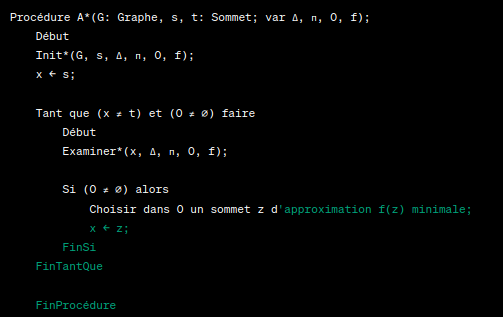
\includegraphics[scale=0.7]{img/A}
	\caption{Algorithme A* }
	\label{Algorithme A*}
\end{figure}


\section{Implémentation des stratégies de jeu}
	\subsection{MinMax}
	L'algorithme minimax est une technique couramment utilisée pour prendre des décisions dans les jeux à deux joueurs, où l'objectif est de maximiser le score du joueur tout en minimisant le score de l'adversaire. L'algorithme explore de manière récursive l'arbre des possibilités de jeu jusqu'à une certaine profondeur (définie par la variable "difficulte" dans le code) pour évaluer chaque position possible.
	
	Le code utilise la récursivité pour simuler les mouvements possibles du joueur et de l'adversaire, en évaluant la valeur de chaque position grâce à une fonction d'évaluation (non fournie dans le code). Il utilise également l'élagage alpha-bêta pour réduire le nombre de branches explorées, ce qui permet d'améliorer les performances de l'algorithme en évitant d'explorer les branches qui n'apporteront pas de meilleures solutions.
	
	
	La méthode "executeAlgo()" lance l'exécution de l'algorithme minimax en appelant la méthode récursive "m()". La valeur retournée par "executeAlgo()" représente le score optimal calculé par l'algorithme, qui est utilisé pour prendre la décision de jeu.
	
	
	\subsection{NégaMax}
	L'idée principale de l'algorithme NegaMax est de minimiser le nombre de lignes de code en utilisant la propriété suivante : la valeur minimax d'un nœud est égale à la négation de la valeur minimax de son nœud enfant avec la meilleure valeur. Cela permet d'éviter d'avoir à implémenter séparément les fonctions Min et Max de l'algorithme MiniMax.
	
	Dans la classe NegaMAXStrategy, la méthode executeAlgo() est appelée pour exécuter l'algorithme NegaMax. Elle renvoie le score obtenu à partir de l'appel initial à la fonction negamax().
	La fonction negamax() est récursive et utilise une approche de recherche en profondeur avec une évaluation heuristique pour évaluer les positions du jeu. Elle prend en compte la profondeur actuelle de la recherche, la position du joueur, le plateau de jeu et la couleur actuelle. Elle évalue les différents coups possibles en appelant récursivement negamax() sur les positions suivantes et en inversant la couleur.

	La fonction endGame() de la classe Board est utilisée pour vérifier si le jeu est terminé ou si la profondeur maximale de recherche a été atteinte.
	
	La fonction eval() est utilisée pour évaluer la position du joueur à partir d'un ensemble de critères spécifiques à Othello, tels que le nombre de coups possibles et le score matériel du joueur.
	
	\subsection{AlphaBeta}
	L'algorithme Alpha-Bêta est une amélioration de l'algorithme Minimax qui permet de réduire le nombre de nœuds évalués. Il effectue une exploration de l'arbre de jeu de manière similaire à l'algorithme Minimax, mais il utilise deux valeurs, alpha et beta, pour effectuer une élagage des branches inutiles.
	
	Dans la méthode alphabeta, l'algorithme Alpha-Bêta est implémenté de manière récursive. Les paramètres alpha et beta représentent respectivement les meilleures valeurs connues pour le joueur maximisant (le joueur courant) et le joueur minimisant (l'adversaire). L'idée est de mettre à jour ces valeurs à chaque niveau de l'arbre pour élaguer les branches qui n'apporteront pas de meilleures solutions.
	
	L'algorithme Alpha-Bêta effectue une recherche en profondeur, en évaluant les positions possibles jusqu'à une certaine profondeur (définie par la variable difficulte). Lorsqu'il est dans un nœud de jeu terminal ou atteint la profondeur maximale, il utilise une fonction d'évaluation (non fournie dans le code) pour attribuer une valeur à cette position.
	
	La méthode executeAlgo() lance l'exécution de l'algorithme Alpha-Bêta en appelant la méthode récursive alphabeta(). La valeur retournée par executeAlgo() représente le score optimal calculé par l'algorithme, qui est utilisé pour prendre la décision de jeu.
	\subsection{NégaAlphaBéta}
	L'algorithme NegaAlphaBeta est une variation de l'algorithme Alpha-Bêta qui utilise la recherche de coup principal (Principal Variation Search) pour améliorer les performances. Il s'agit d'une technique de recherche basée sur la recherche sélective des coups les plus prometteurs.
	
	Dans la méthode negaAlphaBeta, l'algorithme NegaAlphaBeta est implémenté de manière récursive. Les paramètres alpha et beta représentent les meilleures valeurs connues pour le joueur maximisant (le joueur courant) et le joueur minimisant (l'adversaire), respectivement. La variable color est utilisée pour inverser les scores en fonction du joueur courant.
	
	L'algorithme effectue une recherche en profondeur similaire à Alpha-Bêta, en évaluant les positions possibles jusqu'à une certaine profondeur (définie par la variable difficulte). Lorsqu'il est dans un nœud de jeu terminal ou atteint la profondeur maximale, il utilise une fonction d'évaluation (non fournie dans le code) pour attribuer une valeur à cette position.
	
	La méthode executeAlgo() lance l'exécution de l'algorithme NegaAlphaBeta en appelant la méthode récursive negaAlphaBeta(). La valeur retournée par executeAlgo() représente le score optimal calculé par l'algorithme, qui est utilisé pour prendre la décision de jeu.
	\subsection{SSS*}
	Dans le contexte du jeu, cette stratégie qui utilise l'algorithme SSS* pour trouver le meilleur coup à jouer dans le jeu Othello. L'algorithme explore l'arbre des coups possibles jusqu'à une certaine profondeur (définie par la variable difficulte).
	
	La classe SSSStrategy hérite de la classe Strategy et implémente la méthode executeAlgo() qui lance l'algorithme SSS*. La classe contient également une classe interne Node qui représente un nœud de l'arbre de recherche.
	
	L'algorithme SSS* est basé sur une recherche en profondeur itérative. Il utilise une table de hachage (HashMap) appelée nodes pour stocker les nœuds déjà visités et éviter la répétition de calculs. L'algorithme maintient également un chemin (currentPath) de nœuds actuels pour garder une trace de la position courante.
	
	L'algorithme executeAlgo() initialise le nœud current avec la position actuelle du jeu. Ensuite, il itère indéfiniment et effectue la recherche en appelant la méthode search() sur le nœud current. L'algorithme met à jour la meilleure valeur (bestValue) du nœud en fonction des résultats de la recherche. La boucle continue jusqu'à ce qu'une condition de sortie soit satisfaite.
	
	La méthode search() effectue la recherche récursive en explorant les nœuds enfants du nœud courant. Elle utilise la fonction expand() pour étendre les nœuds enfants à partir des successeurs possibles de la position actuelle du jeu. L'algorithme utilise la fonction d'évaluation eval() pour attribuer une valeur à chaque nœud en fonction de certaines heuristiques spécifiques au jeu Othello.

	


\section{Document technique}

\subsection{Fenêtre de démarrage du jeu}
	
		\begin{figure}[H]
		\centering
		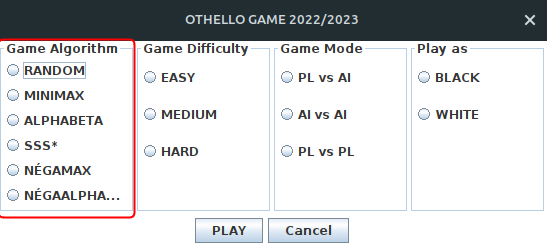
\includegraphics[scale=0.7]{img/algo.png}
		\caption{Choix d'algorithme }
		\label{Algo}
	\end{figure}

	\begin{figure}[H]
	\centering
	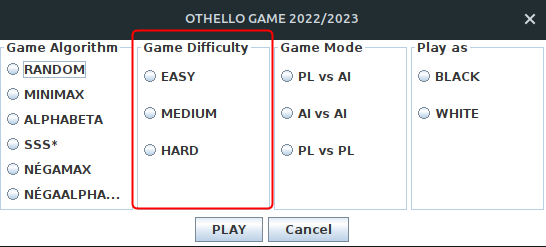
\includegraphics[scale=0.7]{img/diff.png}
	\caption{Choix de niveau }
	\label{niveau}
\end{figure}

	\begin{figure}[H]
	\centering
	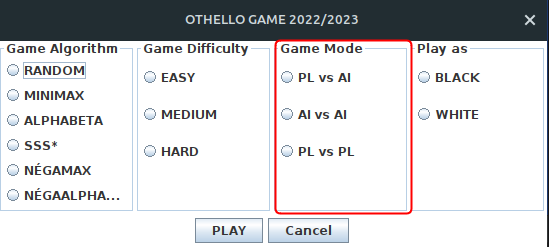
\includegraphics[scale=0.7]{img/mode.png}
	\caption{Choix de mode }
	\label{mode}
\end{figure}

	\begin{figure}[H]
	\centering
	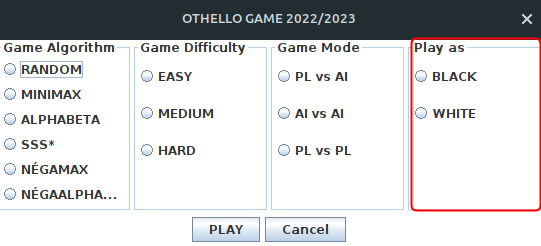
\includegraphics[scale=0.7]{img/joueur.png}
	\caption{Choix de type de joueur }
	\label{joueur}
\end{figure}
	
		\begin{figure}[H]
		\centering
		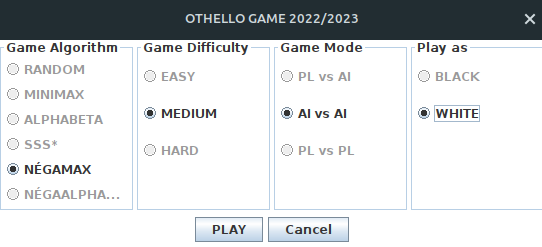
\includegraphics[scale=0.7]{img/choix.png}
		\caption{Exemple d'un choix terminal }
		\label{choix}
	\end{figure}

\subsection{Configurations du jeu}

\subsubsection{Configuration initial du jeu }
 Le plateau de jeu est un carré de 8x8 cases.
Les cases du plateau sont alternativement vides ou contiennent un pion de couleur noire ou blanche.
Au centre du plateau, les 4 cases centrales sont occupées par 2 pions noirs et 2 pions blancs, disposés en croix.\\
    Le joueur blanc a ses pions aux positions (4, 5) et (5, 4).\\
Le joueur noir a ses pions aux positions (4, 4) et (5, 5).
		\begin{figure}[H]
		\centering
		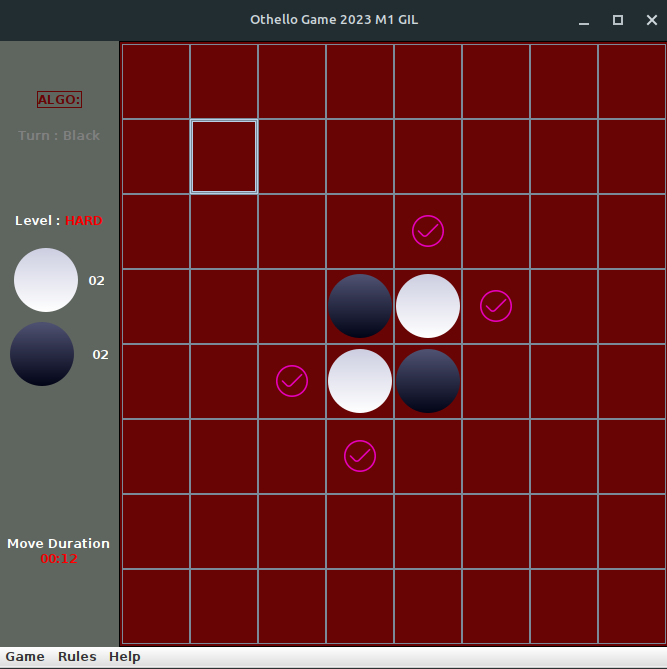
\includegraphics[scale=0.5]{img/conf_init.png}
		\caption{Configuration initial }
		\label{Conf_initial}
	\end{figure}

\newpage
\subsubsection{Menu déroulant}
\textbf{Menu déroulant "Rules":}\\
Lorsque l'utilisateur sélectionne cette option, affichez une nouvelle fenêtre qui présente les règles du jeu Othello.

\textbf{Menu déroulant "Help":}\\
Lorsque l'utilisateur sélectionne cette option, affichez une nouvelle fenêtre qui fournit des informations d'aide sur le jeu.

\textbf{Menu déroulant "Game":}\\ 
\textbf{Sous-menu "Pause":} Lorsque l'utilisateur sélectionne cette option, mettez le jeu en pause. Cela peut être réalisé en arrêtant temporairement la mise à jour du plateau de jeu et en désactivant les interactions avec les pions.\\
\textbf{Sous-menu "Exit":} Lorsque l'utilisateur sélectionne cette option, affichez une fenêtre contextuelle de confirmation pour confirmer si l'utilisateur souhaite vraiment quitter le jeu. Si l'utilisateur confirme, fermez l'application ou revenez à l'écran d'accueil.\\
\textbf{Sous-menu "New Game":} Lorsque l'utilisateur sélectionne cette option, affichez une fenêtre contextuelle de confirmation pour confirmer si l'utilisateur souhaite vraiment recommencer la partie. Si l'utilisateur confirme, réinitialisez le plateau de jeu avec la configuration initiale et redémarrez la partie.

	\begin{figure}[H]
	\centering
	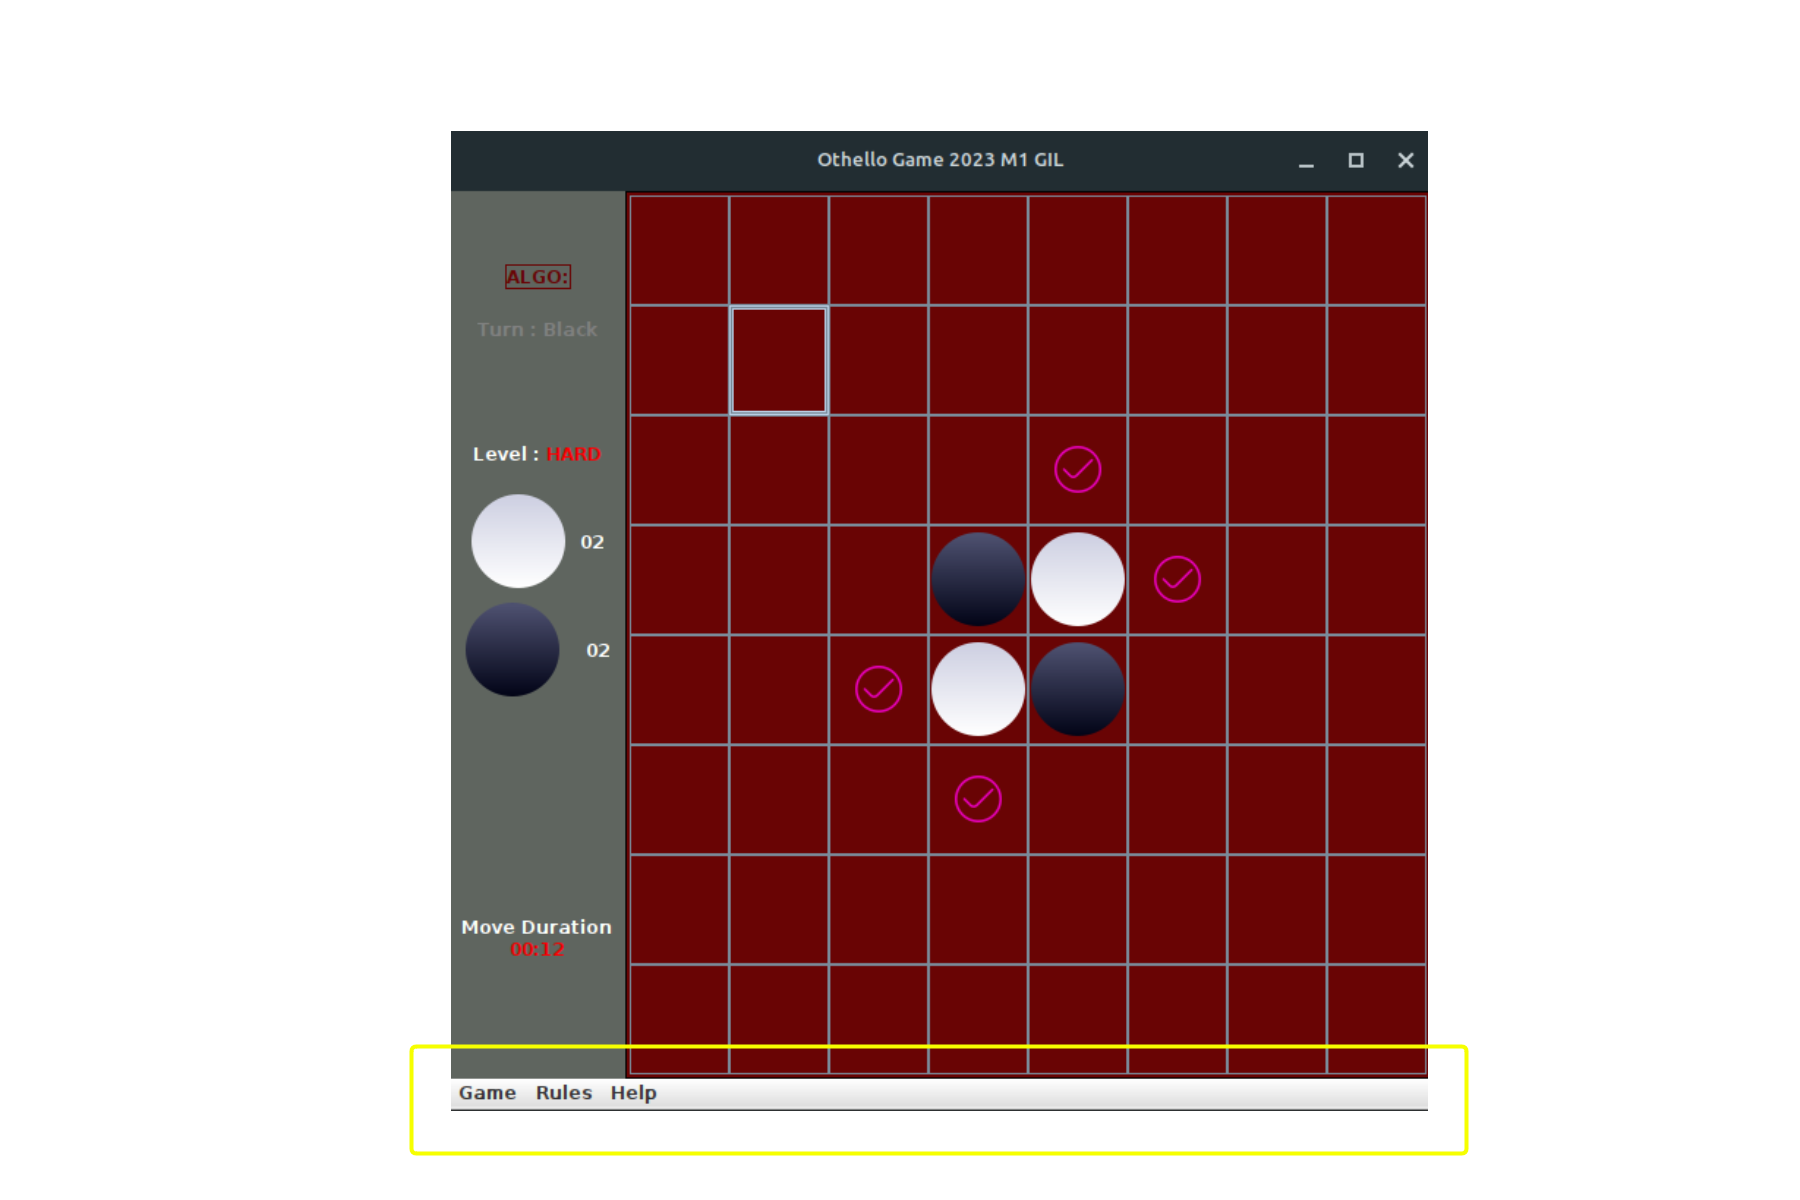
\includegraphics[scale=0.3]{img/rule.png}
	\caption{Menu bar pour l'aide et règles de jeu}
	\label{rules_aide}
\end{figure}

\subsubsection{Zone Partie}
Dans cette zone on a toutes les informations concernant notre partie telque:
L'algorithme choisi , le score pour chaque joueur , le niveau choisi, le tour , et le temps de mouvement .

	\begin{figure}[H]
	\centering
	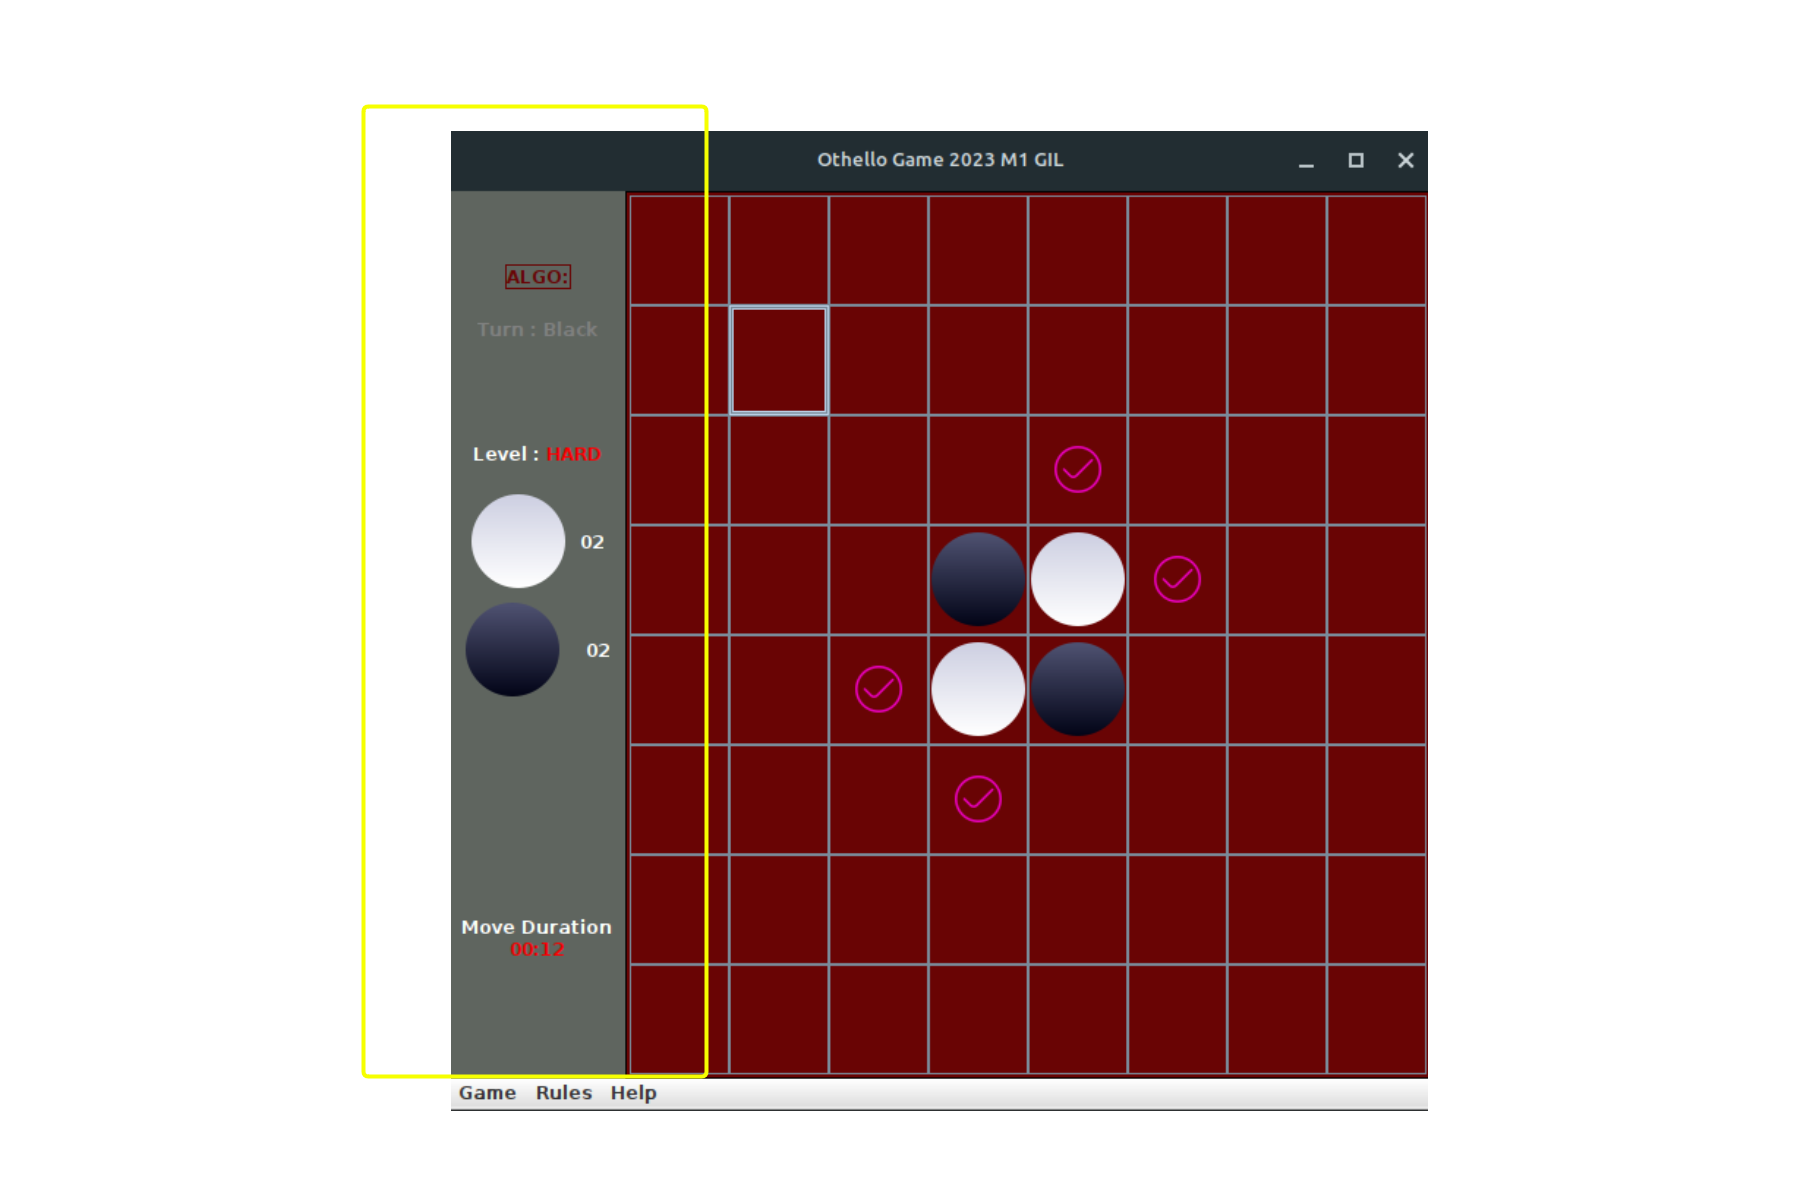
\includegraphics[scale=0.3]{img/pion.png}
	\caption{Informations de la partie}
	\label{pion}
\end{figure}

\subsubsection{Zone du jeu principale}

\paragraph{Affichage des cases conviviales :}

Analysez l'état actuel du jeu pour déterminer les cases conviviales pour le joueur en cours.\\
Marquez visuellement ces cases conviviales d'une manière distinctive, par exemple dans notre cas on a utilisé des icons comme un indicateur visuel.
\paragraph{Gestion des cases non conviviales :}

Si le joueur clique sur une case qui n'est pas conviviale,le clique est ignoré pour informer le joueur que le mouvement n'est pas autorisé.
Le joueur devra alors sélectionner une case conviviale valide pour effectuer son mouvement.
	\begin{figure}[H]
	\centering
	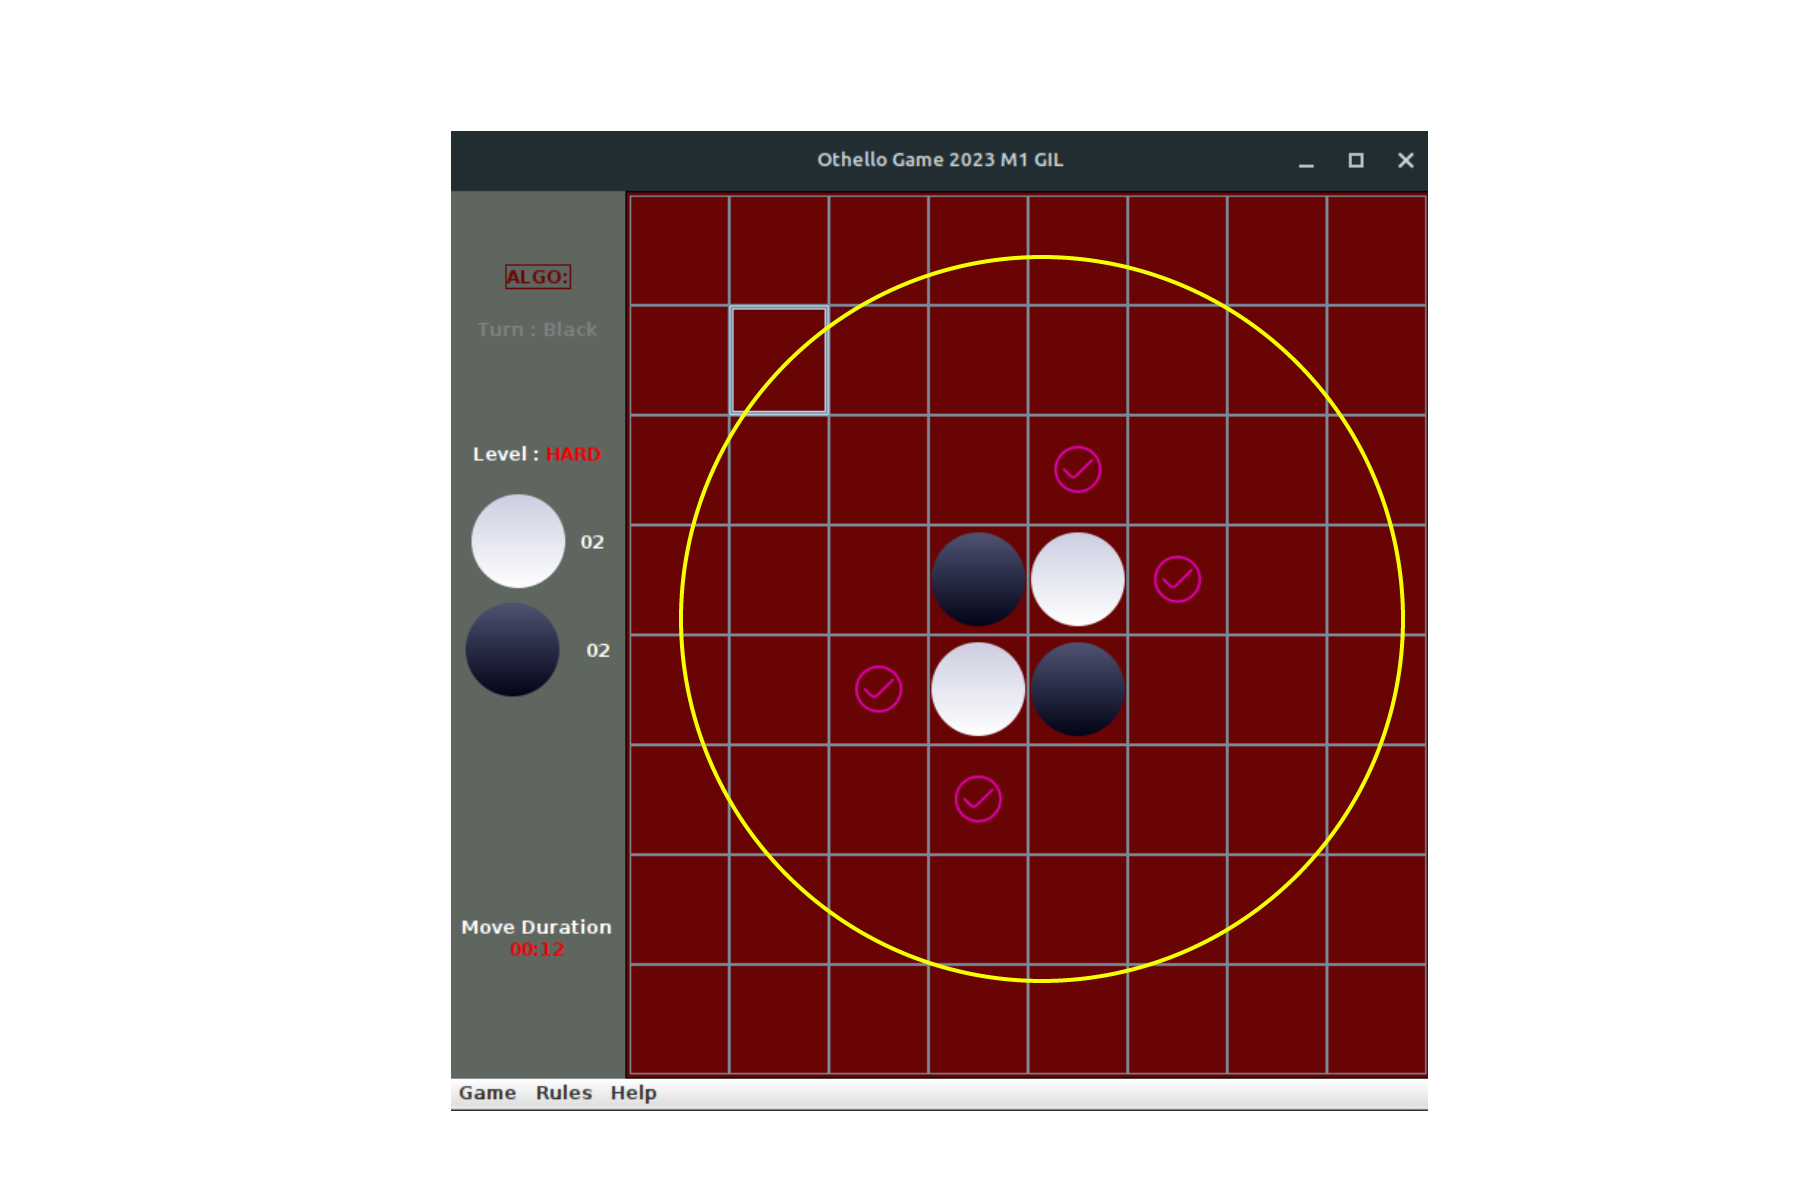
\includegraphics[scale=0.3]{img/zone.png}
	\caption{Zone de jeu}
	\label{zone}
\end{figure}
	
	
	
	
	
	
	
	
	
	
	
	
	
	
	
	
	
	
	
	
	
	
	
	
	
	
	%---------------------------------Fin de rapport---------------------------
	\section{Conclusion}
En conclusion, notre projet a consisté à réaliser le jeu Othello en Java en utilisant différents algorithmes de stratégies de jeu tels que MinMax, AlphaBeta, NegAlphaBeta, SSS* et A* malheureusement on à réussi à implémenté que les 4 premiers . Nous avons implémenté les règles du jeu et avons offert la possibilité aux joueurs de choisir leur niveau de difficulté ainsi que leur mode de jeu \textbf{(joueur contre joueur, joueur contre ordinateur, ordinateur contre ordinateur)}. Pour être efficaces, nous avons basé l'utilisation de ces algorithmes sur une analyse correcte du jeu. Ce projet nous a permis de renforcer nos compétences en programmation orientée objet ainsi que notre compréhension de l'utilisation des algorithmes pour la résolution de problèmes.
\end{document}